%\usepackage{lipsum}

\documentclass[12pt]{article}
\usepackage[english]{babel}
\usepackage[utf8]{inputenc}
\usepackage{fancyhdr}
\usepackage{graphicx}
\usepackage{helvet} %set font to arial like 
\renewcommand{\familydefault}{\sfdefault}
\usepackage[table]{xcolor} %coloring the tables
\usepackage[font=small,labelfont = bf]{caption} %set the fontsize of the captions in arial font
\usepackage{siunitx} %standard si unit package
\usepackage{adjustbox} %adjustbox to position the table, probably unnecessary yet handy
\usepackage[margin = 0.2cm]{subcaption} %fine tuning of possible subfigures
\usepackage[a4paper, margin=1.5cm,headsep = 0.1in,tmargin = 1.5in,headheight = 72pt]{geometry}%geometry package margin sets left/right border, headsep sets distance from header to text, t margin distance top of text to page, headheight is necessary for multiline headers 
%\usepackage[no-math]{fontspec} %for the lulz if you dare
%\setmainfont[BoldFont = LDFComicSansBold]{LDFComicSans}
%\usepackage{mathtools}
%\usepackage{unicode-math}
%\setmathfont{Latin Modern Math}
\pagestyle{fancy} %package used for the headers
\fancyhf{}
%%%%%%%%%%%%%%%%%%%%%%%%%%%%%%%%%%%%%%%%%%%%%%%%%%%%%%%%%%%%%%%%%%%%%%%%%%
%Standard header for the measurement reports
\rhead{\footnotesize \textbf{Heinz Maier-Leibnitz Zentrum}\\
\textbf{User Office}\\
Lichtenbergstr. 1, 85748 Garching/Germany\\
Phone: +49.(0)89.10703/10794\\
Fax: +49.(0)89.10799\\
\textbf{
Email: useroffice@mlz-garching.de  	Web: mlz-garching.de/user-office}}
\lhead{
\includegraphics[width=3.25cm]{mlz}\\}
\renewcommand{\headrulewidth}{0pt}
%%%%%%%%%%%%%%%%%%%%%%%%%%%%%%%%%%%%%%%%%%%%%%%%%%%%%%%%%%%%%%%%%%%%%%%%%%
\renewcommand{\arraystretch}{1.5}
\newcolumntype{g}{>{\columncolor[HTML]{cccccc}} p{0.25\textwidth}}
\setlength{\arrayrulewidth}{0mm}
\definecolor{lightgray}{RGB}{204, 204, 204}
\usepackage{etoolbox}
\patchcmd{\thebibliography}{\section*{\refname}}{}{}{}
\begin{document}
%%%%%%%%%%%%%%%%%%%%%%%%%%%%%%%%%%%%%%%%%%%%%%%%%%%%%%%%%%%%%%%%%%%%%%%%%%%%

% Leading table collecting general information about the experiment

\begin{table}[h]
	\begin{adjustbox}{width=1\textwidth}
		\begin{tabular}{ |g|p{0.72\textwidth}|  }
			\arrayrulecolor{darkgray}
			\hline
			\rowcolor{lightgray} \multicolumn{2}{|l|}{\textbf{\large
					EXPERIMENTAL REPORT}} \\
			\hline
			\rowcolor{lightgray} \multicolumn{2}{|l|}{\textbf{\large Experiment Title}} \\
			\hline
			\multicolumn{2}{|l|}{
			 
			} \\[-3ex]
			\multicolumn{2}{|l|}{
				%%%%%%%%%%%%%%%%%%%%%%%%%%%%%%%%%%%%%%%%%%%%%%%%%%%%%%%%%%%%
				Nested-mirror optic: A novel type of focusing optic for MIEZE
				
				%%%%%%%%%%%%%%%%%%%%%%%%%%%%%%%%%%%%%%%%%%%%%%%%%%%%%%%%%%%%
			} \\[1ex]
			\hline
			%%%%%%%%%%%%%%%%%%%%%%%%%%%%%%%%%%%%%%%%%%%%%%%%%%%%%%%%
			\textbf{Proposal number}   & 16334\\ \hline
			\textbf{Instrument} & MIRA\\ \hline
			\textbf{Date of Experiment} &29/01/2020 – 03/02/2020\\ \hline
			\textbf{Local Contact}    &Robert Georgii\\ 
			%%%%%%%%%%%%%%%%%%%%%%%%%%%%%%%%%%%%%%%%%%%%%%%%%%%%%%%%
			
			\hline
			\rowcolor{lightgray} \multicolumn{2}{|l|}{\textbf{Experimental Team}} \\
			\hline
			\multicolumn{2}{|l|}{
				%%%%%%%%%%%%%%%%%%%%%%%%%%%%%%%%%%%%%%%%%%%%%%%%%%%%%
				Christoph Herb$ ^{1} $, Oliver Zimmer $ ^{2} $, Peter Böni $ ^{1} $
				%%%%%%%%%%%%%%%%%%%%%%%%%%%%%%%%%%%%%%%%%%%%%%%%%%%%%
			} \\
			\hline
			\rowcolor{lightgray}\multicolumn{2}{|l|}{\textbf{Affiliations}} \\
			\hline
			\multicolumn{2}{|l|}{$ ^{1} $Physics Department, E21 Technical University Munich} \\[-1ex]
			\hline
			\multicolumn{2}{|l|}{$ ^{2} $Institut Laue-Langevin}\\
			\hline
		\end{tabular}
	\end{adjustbox}
\end{table}
%%%%%%%%%%%%%%%%%%%%%%%%%%%%%%%%%%%%%%%%%%%%%%%%%%%%%%%%%%%%%%%%%%%%%%
\noindent
\textbf{Sample:}\newline
We investigated a novel type neutron optic described by Oliver Zimmer \cite{zimmer18} and provided by Peter Böni with emphasis on the focusing properties and the efficiency of the optical device. Further investigations concerning the errors introduced by a misalignment of the optic with respect to the optical axis are planned. Theoretical considerations concerning the novel nested optic can be found in \cite{zimmer16}.\\
\textbf{Experiment:}\newline
During the measurement, the nested optic was oriented on the sample table of the instrument allowing to precisely control the angle of incidence. Close up images of the optic including the scale and a sketch of the used measurement geometry up are shown in figure \ref{fig:theoptic}.\\
\begin{figure}[h]
	\centering
	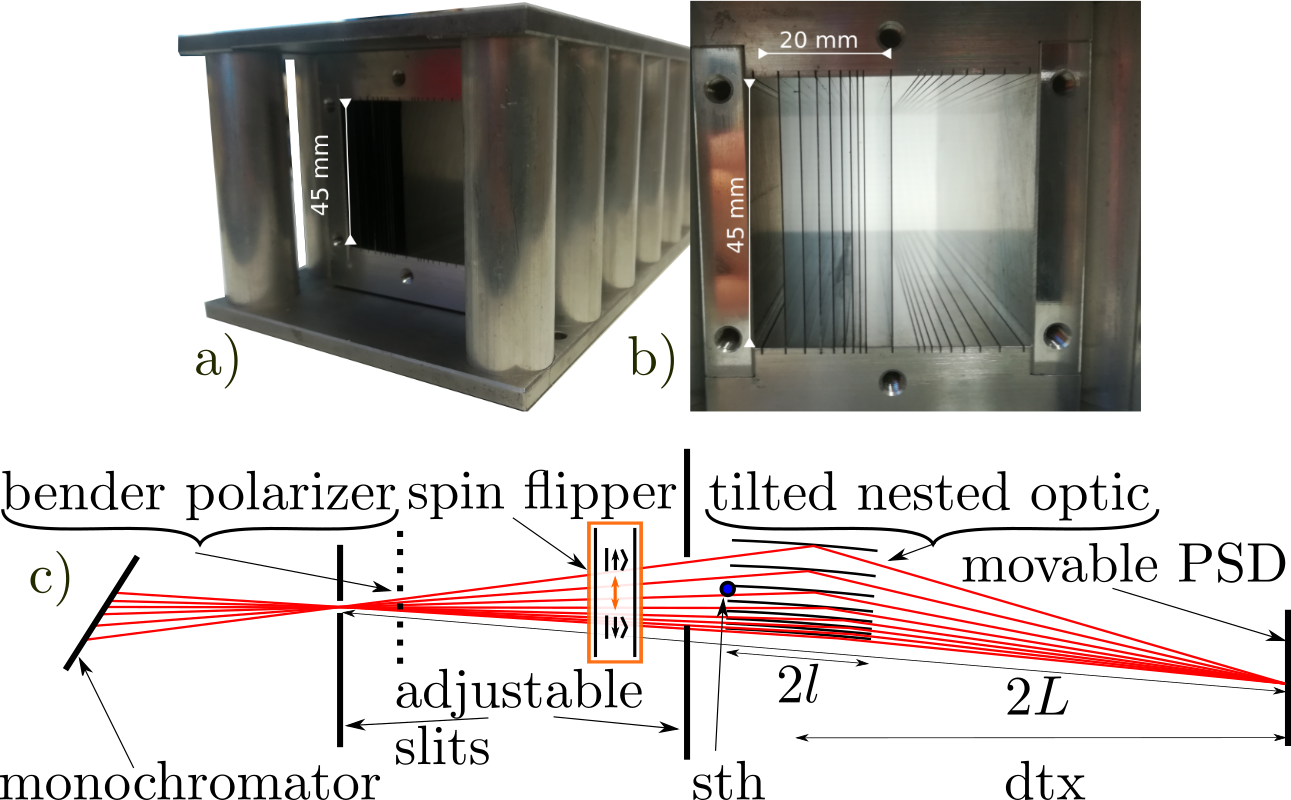
\includegraphics[width=.56\textwidth]{./figures_report/mirameasboth}
	\caption{a) Image of the polarizing neutron optic with the dimensions of the channel. b) Shows the 8 individual polarizing mirrors on the left side of the optic and the central mirror solely used for orientation. c) depicts a top view of the experimental setup including two adjustable slits, the bender polarizer, the spin flipper, the movable position sensitive detector (PSD) and the optic sitting on the sample stage. }
	\label{fig:theoptic}
\end{figure}
While the device was prepared to host a symmetric mirror assembly (including the empty slits in figure \ref{fig:theoptic} b), we resorted to using only half of the available mirrors for our experiment, resulting in the geometry shown in figure \ref{fig:theoptic} c). The neutrons coming from the monochromator were fed through the first of the adjustable slits before being polarized by a bender polarizer consisting of horizontally arranged, curved mirrors. A spin flipper allowed to reverse the spin of the neutrons thereafter. The optic was oriented in such a way that one focal point is located at the center of the first slit. Its width limits the resolution of the image observed behind the optic. The second slit directly in front of the optic served to define an entrance window for the incident beam, cutting the angular range to fit the mirror system.  Finally, an image of the reflected neutrons was acquired by using the position sensitive detector (PSD). The PSD was freely movable along the neutron flight path to investigate both, the beam at the point of maximum focus and the degree of blurring introduced by being beside the maximum. The neutron polarization generated by the bender was maintained by a guide field applied on the whole path between the bender and the polarizing mirror optic. The additional degree of freedom of neutron polarization turned out to be quite useful to identify the origin of different components of the images with the help of the spin flipper .\\
In summary, the experiment successfully demonstrated the performance of the nested optic in good agreement with previous simulations. Figure \ref{fig:allthree} presents exemplary images showing the leakage of the neutrons between the nested mirrors at low angles, a perfectly focused neutron beam and double reflections occurring when the optic is tilted beyond the ideal angle.
\begin{figure}[y]
	\centering
	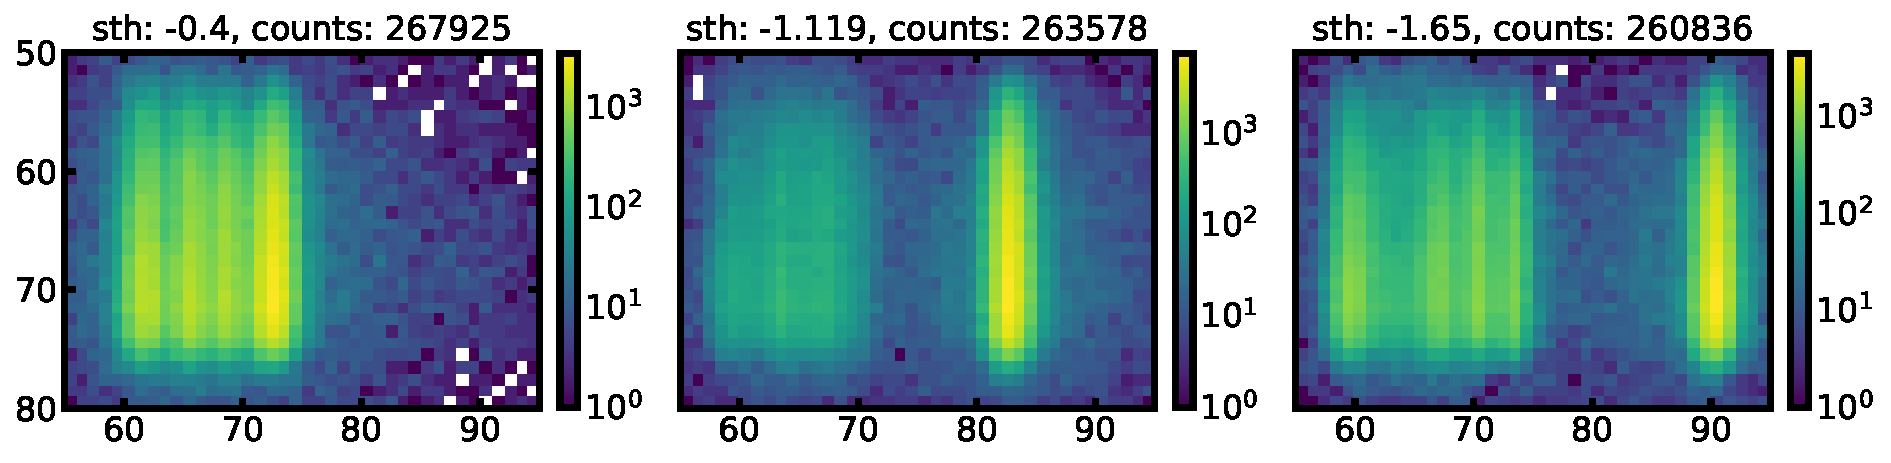
\includegraphics[width=1\textwidth]{./figures_report/focus}
	\caption{Subset of the acquired image with the detector in an optimal focusing distance. The images show the neutron distribution at the focus position for differently rotated neutron optics. At small angles (sth: $\SI{-0.4}{^\circ}$), a portion of the neutrons passes between the blades of the mirrors unhindered. The projection of the mirrors is clearly visible as shadows on the detector. In perfect focusing (sth: $\SI{-1.119}{^\circ}$), the intensity of reflected neutrons is very pronounced and intense, while the diffuse background visible in the direct path of the neutrons is very low and diffuse. This intensity is generally attributed to neutrons in the wrong state of polarization. The third image taken at an angle larger than optimal, shows the focused neutrons further to the right as the optic is tilted. At the direction of the direct beam path, intensities arising from double reflections appear in accordance with theory. The total neutron counts on the whole detector decrease only slightly with increasing tilt angle, which indicates that few neutrons are lost as a result of the reflection processes.}
	\label{fig:allthree}
\end{figure}

\noindent\textbf{Outlook}:
The efficiency of the full optic has to be investigated further in a geometry more similar to the proposed MIEZE experiment. This also requires testing whether simultaneous focusing in horizontal and vertical direction is feasible. Further trials also include non-polarizing blades simplifying the geometry by allowing to dismiss the polarizer and the guide fields.

\bibliographystyle{alpha}
\bibliography{measurement_report.bib}
\end{document}

